\section{Game Combat Model}

\subsection{Modeling}
To be able to search over possible future states of the game it is necessary to be able to represent such future states,
and since is not possible to try the outcomes of different actions through the \textsc{Starcraft} engine, 
we must create a model of the game and simulate this separately.
A similar model is presented in \cite{portfolio} but the one presented here allows for more detailed reproductions of all of the timings and various intricacies of the game engine, possibly at the expense of computation time.
It also allows for modeling things such as splash damage and spells, but does not, at the moment, consider unit collisions.

In order to search for a solution, we created the following components:

\begin{descri}
%STATE
\item[State] $s=<t,U_p,U_e,E,S_A>$:
\begin{shortitem}
\item Current game time $t$
\item Set $U_p$ of the player's units
\item Set $U_e$ of the enemy's units
\item Set of pending effects $E$
\item Set $S_A$ of allowed sets of actions that can be performed from $s$ (multiple units may be be ordered to at the same time)
\end{shortitem}

%UNIT
\item[Unit] $u = <p,hp,b_a,b_m,S_A>$
\begin{shortitem}
\item Position $p = (x,y) \in \mathbb{Z}^2$
\item Current hit points $hp$ ($\Leftrightarrow$ health points)
\item Booleans indicating if the unit can attack $b_a$ or move $b_m$
\item A static set $S_A$ of all possible actions that the unit can perform
\end{shortitem}

There are many different actions, such as: attack, move, deploy, spells, etc.
%ACTION
\item[Action] $a=<pc,E>$
\begin{shortitem}
\item Precondition $pc$ for the action to be allowed in the current gamestate
\item Set $E$ of effects the action will have on the gamestate.
	Most effects are delayed and will not alter the gamestate right away, and will instead be put in the state's set of pending effects $E$.
\end{shortitem}

Effects, in turn, can have various parameters, such as \emph{attacker} and \emph{target} in the case of an attack effect, or \emph{unit} and \emph{direction} in the case of an move effect.
The only things they have in common is that they have an frame offset $t_e$ and that they may modify any part of the gamestate when applied.
%EFFECT
\item[Effect] $e=<t_e>$
\begin{shortitem}
\item Frame offset $t_e$ relative to the frame on which the action it is part of was issued. At this offset the effect is to be applied to the gamestate
\end{shortitem}
\end{descri}

Table \ref{effectUnits} presents the effect corresponding to an attack for two kinds of units (a \texttt{Marine} and a \texttt{Firebat}).
As we can see units' actions have impacts on \emph{future} frames.

\begin{table}[h!t]
    \centering
\subfloat{
\centering
\begin{tabular}{cc|ccc}
&& unit can & Decrease & Weapon in \\
&& not move & $target.hp$ & cooldown \\
\hline
\multirow{4}{*}{\rot{Frame}} 
& 0    & \OK &     & \OK  \\
& 1    & \OK & \OK & \OK  \\
& 2-5  & \OK &     & \OK  \\
& 6-17 &     &     & \OK  \\
\end{tabular}
}
\\
\subfloat{
\centering
\begin{tabular}{cc|ccc}
&& unit can & Decrease & Weapon in \\
&& not move & $target.hp$ & cooldown \\
\hline
\multirow{4}{*}{\rot{Frame}} 
& 0-4   & \OK &     & \OK  \\
& 5-6   & \OK & \OK & \OK  \\
& 7-10  & \OK &     & \OK  \\
& 11-24 &     &     & \OK  \\
\end{tabular}
}
\caption{Exemple of effects $e=<u,target,t_e,type>$}
\label{effectUnits}
\end{table}

\subsection{State generation}

Algorithm \ref{algGeneration} explains how a new state is constructed, taking into account the actions performed to go from the parent to the new child and the pending effects.

\begin{figure}[h!t]
\begin{algorithm}[State generation]
%\begin{descri} 
The following algorithm describes how a new state $s_1=<t,U_p,U_e,E,S_A>$ is constructed from its parent $s_0$ and a set of allowed actions $a$. \ \\
%\end{descri}

\textbf{Function} $descend(s_0,A)$:
\begin{enum}
\item $s_1.t = s_0.t$
\item $s_1.U_p = s_0.U_p$
\item $s_1.U_e = s_0.U_e$
\item $s_1.E = s_0.E \cup A.E$
\item Create the set $s_1.S_A$ of allowed sets of actions available from $s_1$

\item \textbf{While} $S_A$ is empty and no team has won
\begin{enum}
	\item $s_1.t = s_1.t + 1$
	\item apply all effects $\{e \in s_0.E | e.t_e = s_1.t\}$ to $s_1$
	\item $s_1.E = \{e \in s_0.E | e.t_e > s_1.t\}$
	\item Create the set $s_1.S_A$ of allowed sets of actions available from $s_1$
\end{enum}

\item \textbf{Return} $s_1$

\end{enum}
\label{algGeneration}
\end{algorithm}
\end{figure}



\subsection{Allowed actions generation}
The allowed actions for each game state corresponds to which the children of each node are in the game tree.
The problem is only that in RTS games, the number of all allowed actions quickly grows beyond what is feasible to perform an exhastive search on.
Consider that even in as small an battle as that between 10 units, 5 on each team, each having 5 possible actions
(move \texttt{North}, move \texttt{South}, move \texttt{East}, move \texttt{West}, attack
lead to $5^10 = 9765625$ possible combinations of orders only for the first frame.
\footnote{This number is then lower or even zero for subsequent frames while the units are busy executing their given orders, but may grow again when the units are finished.}
Which the allowed actions are for each state depends on the method being used, two possible such methods are:

\begin{shortitem}
\item \texttt{PlayerActionSubset:}
	Taking the huge number of allowed action combinations into account, one way of addressing this issue is to only consider a random subset of them.
\item \texttt{UnitAction:}
	Another way of managing the branches of the tree is to not generate complete combinations of one action for every unit at every level of the tree, but instead only considering the allowed actions of a single unit at each level in the tree.
	This way, it may be possible to prune bad choices for specific units more efficiently, but unless the unit is the one whose's actions are consider at the root of the tree, the same action may be evaluated again in other branches of the tree.
\end{shortitem}

Figure \ref{tree} displays an example of a tree constructed and traversed by the algorithm. Only some nodes of the tree are contructed.
As shown in Algorithm \ref{algGeneration}, a child's frame number is incremented until either a terminal state is reached or any actions become available.
As an example, assuming that our set of actions attributes an attack sequence to each of the \texttt{Marine} in the battleground and according to Table \ref{effectUnits}, there will not be any new actions available until the sixth frame.

\begin{figure}[h!t]
\centering
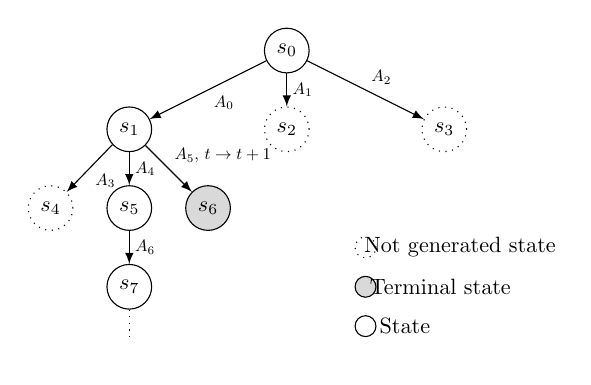
\begin{tikzpicture}[node distance = 1cm]
    \tikzstyle{node}=[circle,align=center,scale=0.8,draw]
    \tikzstyle{nodenotgen}=[circle,dotted,align=center,scale=0.8,draw]
    \tikzstyle{nodeterm}=[circle,fill=gray!30,align=center,scale=0.8,draw]
    \tikzstyle{link}=[->,thin,>=latex]
    
    \node[node] (s0) at (4,4) {$s_0$};

    \node[node] (s1) at (2,3) {$s_1$};
    \node[nodenotgen] (s2) at (4,3) {$s_2$};
    \node[nodenotgen] (s3) at (6,3) {$s_3$};

    \node[nodenotgen] (s4) at (1,2) {$s_4$};
    \node[node] (s5) at (2,2) {$s_5$};
    \node[nodeterm] (s6) at (3,2) {$s_6$};

    \node[node] (s7) at (2,1) {$s_7$};

    \node[auto,scale=0.8] (s8) at (2,0.2) {};
    
    \draw[link] (s0) to node [auto,scale=0.6] {$A_0$} (s1); 
    \draw[link] (s0) to node [auto,scale=0.6] {$A_1$} (s2);
    \draw[link] (s0) to node [auto,scale=0.6] {$A_2$} (s3);
    \draw[link] (s1) to node [auto,scale=0.6] {$A_3$} (s4);
    \draw[link] (s1) to node [auto,scale=0.6] {$A_4$} (s5);
    \draw[link] (s1) to node [auto,scale=0.6] {$A_5$, $t \rightarrow t+1$} (s6);
    \draw[link] (s5) to node [auto,scale=0.6] {$A_6$} (s7);
    \draw[-,>=latex,dotted] (s7) to (s8);
    

    %LEGEND

    \node[node] (l1) at (5,0.5) {}; % {$\phantom{s_1}$};
    \node[nodeterm] (l2) at (5,1)  {}; %{$\phantom{s_1}$};
    \node[nodenotgen] (l3) at (5,1.5) {}; %{$\phantom{s_1}$};
    \node[align=left,rectangle,scale=0.8] (l1t) at (5.5,0.5) {State};
    \node[align=left,rectangle,scale=0.8] (l2t) at (5.95,1.0) {Terminal state};
    \node[align=left,rectangle,scale=0.8] (l3t) at (6.2,1.5) {Not generated state};

\end{tikzpicture}
\caption{Exemple of a tree}
\label{tree}
\end{figure}



\subsection{Move ordering}
After selecting which are the allowed sets of actions from each state, that is, the children of each node in the game tree, it is of further interest to prune the less promising branches of the tree.
For this, move ordering, or deciding in which order to evaluate the children, is important since it allows for earlier pruning.
The time restriction of RTS games greatly limits the maximum number of childs that can be explored, and it is well known that a good move ordering can greatly improve performance.

One interesting way of doing this is presented in \cite{portfolio}.
Their idea is to first consider the actions produced by some scripted behaviors that generally perform quite good.



\subsection{State evaluation}
For comparing how good states are, it is necessary to make use of some evaluation function.
The evaluation functions suggested by \cite{abcd} are the following:
\begin{shortitem}
\item Straight Forward Evaluations:
$$
    \displaystyle{SFE(s) = \sum_{u \in s.U_p} u.hp - \sum_{u \in s.U_e} u.hp } 
$$

\item Life Time Damage:
$$
    \displaystyle{LTD(s) = \sum_{u \in s.U_p} u.hp \cdot u.DPS- \sum_{u \in s.U_e} u.hp \cdot u.DPS } 
$$

\item Life Time Damage 2:
$$
    \displaystyle{LTD2(s) = \sum_{u \in s.U_p} \sqrt{u.hp} \cdot u.DPS - \sum_{u \in s.U_e} \sqrt{u.hp} \cdot u.DPS } 
$$

\item Playouts:
	Another way of evaluating the state commonly used in Monte Carlo Tree Search algorithms is playouts. In essence the game state is played out to a terminal state either by picking random moves for the players or by using some scripted behaviors.
\end{shortitem}


$SFE$ doesn't take into account units' damage per second, DPS -- which is an essential information during a battle. 
$LTD$ present a good estimation of DPS but does not favor equal hit point distribution among the units. 
Ultimately $LTD2$ measures the DPS and favor the greatest number of units remaining\footnote{Having two units with $50$ hit points means higher DPS than one with $100$ hit points.}.




